Consider the positive-feedback circuit shown in Fig. \ref{fig:ee18btech11030}. 
\begin{figure}[!ht]
	\begin{center}
		\resizebox{\columnwidth/1}{!}{ 
\usetikzlibrary{decorations.markings}
\begin{circuitikz}
\draw (-4,-1) to[amp,t={+K}] (2.5,-1);
\draw (-4,-1) to (-4,2) to (-3,2) ;
\draw (-3,2)  to [capacitor=$C/10$](-3,0.5) to  (-3,0.5) node[ground]{};
\draw (-3,2) to (-2.3,2)to [R=$10R$] (-1.3,2)to (0,2) to [R=$R$] (0,5) node[label={}]{}  to (-4,5) ;
\draw (0,2) to(1,2) to  [capacitor=$C$](1.5,2) to (2.5,2) to (2.5,-1);
\draw (-4,5) to (-4,4.7) to [V=$V_s$] (-4,3.9) to (-4,3.5) node[ground]{} ;
\draw (2.5,-1) to[short, -o] (3,-1) node[label={above:$V_{out}$}]{};
\end{circuitikz}}
	\end{center}
	\caption{ Positive Feedback Circuit}
	\label{fig:ee18btech11030}
\end{figure}
\begin{enumerate}[label=(\alph*),ref=\theenumi]

\item Find the loop transmission L(s) and the characteristic equation ,find the expressions for resulting pole frequency $\omega_o$ and Q factor?
\item Sketch a Pole-Zero plot for varying K. 
\item For what value of K do the poles coincide? For what value of K does the response becomes maximally flat? For what value of K does the circuit oscillate?
\end{enumerate}
Assume that the amplifier has frequency-independent gain, infinite input impedance, and zero output impedance.
%\begin{enumerate}[label=\thesubsection.\arabic*.,ref=\thesubsection.\theenumi]
\begin{enumerate}[label=\arabic*.,ref=\theenumi]
\numberwithin{equation}{enumi}
\item Find $L(s)$.

\solution To obtain the loop transmission L(s),
\begin{itemize}
\item Short-circuit the signal source $V_s$.
\item Break the loop at the Amplifier input.
\item Then apply a test voltage $V_t$ and find the returned voltage $V_r$, as indicated in Figure: \ref{fig:ee18btech11030_fig1}.
\end{itemize}

\begin{figure}[!ht]
	\begin{center}
		\resizebox{\columnwidth/1}{!}{\usetikzlibrary{decorations.markings}
\begin{circuitikz}
\draw (-2,0) to[amp,t={+K}] (3,0);
\draw (3,0) to (3,4) to [capacitor=$C$](1.7,4) to (1,4)  to [R=$R$] (1,2) to (1,2) node[ground]{} ;
\draw (3,4) to [short, -o] (3.5,4) node[label={above:$V_{1}$}]{} ;
\draw [dashed] (2.8,1) to (-1.5,1) to (-1.5,4.5) to (2.8,4.5) to (2.8,1); 
\draw (1,4) to  [R=$10R$] (-1,4) to [capacitor=$C/10$](-1,2) to (-1,2) node[ground]{} ;
\draw (-1,4) to [short, -o] (-2,4) node[label={above:$V_{r}$}]{};
\draw (-2,0) to [short, -o] (-3,0) node[label={above:$V_{t}$}]{} ;
\end{circuitikz}
}
	\end{center}
	\caption{}
	\label{fig:ee18btech11030_fig1}
\end{figure}

The loop transmission is given by
\begin{align}
    L\brak{s} = -\frac{V_r\brak{s}}{V_t\brak{s}} = -KT\brak{s}
\label{eq:ee18btech11030}
\end{align}
where T(s) is the transfer function of the two-port RC network shown inside the broken-line box in Figure: \ref{fig:ee18btech11030_fig1}.

\begin{align}
T\brak{s} = \frac{V_r\brak{s}}{V_1\brak{s}}
\label{eq:ee18btech11030_1}
\end{align}
Applying KCL at nodes present in the RC network yields  
\begin{align}
T\brak{s} = \frac{s(\frac{1}{CR})}{s^2 + s(\frac{2.1}{CR}) + (\frac{1}{CR})^2}
\label{eq:ee18btech11030_2}
\end{align}
Substituting T\brak{s} in Eq: \ref{eq:ee18btech11030}
\begin{align}
    L\brak{s} = \frac{-s(\frac{K}{CR})}{s^2 + s(\frac{2.1}{CR}) + (\frac{1}{CR})^2}
\end{align}
The characteristic equation is 
\begin{align}
    1+L\brak{s}=0  
\end{align}
\begin{align}
s^2 + s(\frac{2.1-K}{CR}) + (\frac{1}{CR})^2 = 0
\label{eq:ee18btech11030_3}
\end{align}
The standard characteristic equation of a second order network can be written as 
\begin{align}
    s^2 + \frac{\omega_o}{Q}s + \omega_o^2 = 0
    \label{eq:ee18btech11030_4}
\end{align}
$\omega_o$ is called pole frequency , Q is called pole Qfactor. 
By comparing the Eq:\ref{eq:ee18btech11030_3} with the standard characteristic equation Eq:\ref{eq:ee18btech11030_4}
\begin{align}
   \omega_o = \frac{1}{RC} ; Q = \frac{1}{2.1-K}
\end{align}

\item Equivalent control system model of Fig. \ref{fig:ee18btech11030_fig1}

\solution
\begin{figure}[!ht]
	\begin{center}
		\resizebox{\columnwidth/1}{!}{ 
\tikzstyle{block} = [draw, fill=white!20, rectangle, 
    minimum height=2em, minimum width=6em]
\tikzstyle{sum} = [draw, fill=white!20, circle, node distance=1cm]
\tikzstyle{input} = [coordinate]
\tikzstyle{output} = [coordinate]
\tikzstyle{pinstyle} = [pin edge={to-,thin,black}]

\begin{tikzpicture}[auto, node distance=3cm,>=latex']
    \node [input, name=input] {};
    \node [sum, right of=input] (sum) {};
    \node [block, right of=sum] (controller) {$G(s) = K$};
    \node [output, right of=controller] (output) {};
    \node [block, below of=controller] (feedback) {$H(s) = \frac{1}{sRC + \frac{1}{sRC} + 2.1}$};

    \draw [->] (sum) -- node {$V_i$} (controller);
    \draw [->] (controller) -- node [name=y] {$V_o$}(output);
    \draw [->] (y) |- (feedback);
    \draw [->] (feedback) -| node[pos=0.99]{$+$}  node [near end] {$V_f$} (sum);
\end{tikzpicture}}
	\end{center}
	\caption{ Positive Feedback Circuit}
	\label{fig:ee18btech11030_fig2}
\end{figure}

Closed Loop gain 
\begin{align}
    T = \frac{k(s^2+s(\frac{2.1}{RC})+(\frac{1}{RC})^2)}{s^2 + s(\frac{2.1-K}{CR}) + (\frac{1}{CR})^2}
    \label{eq:ee18btech11030_5}
\end{align}

\item Sketch the Normalised closed loop gain of T for various Q values

\solution 
\begin{figure}[!h]
\centering
  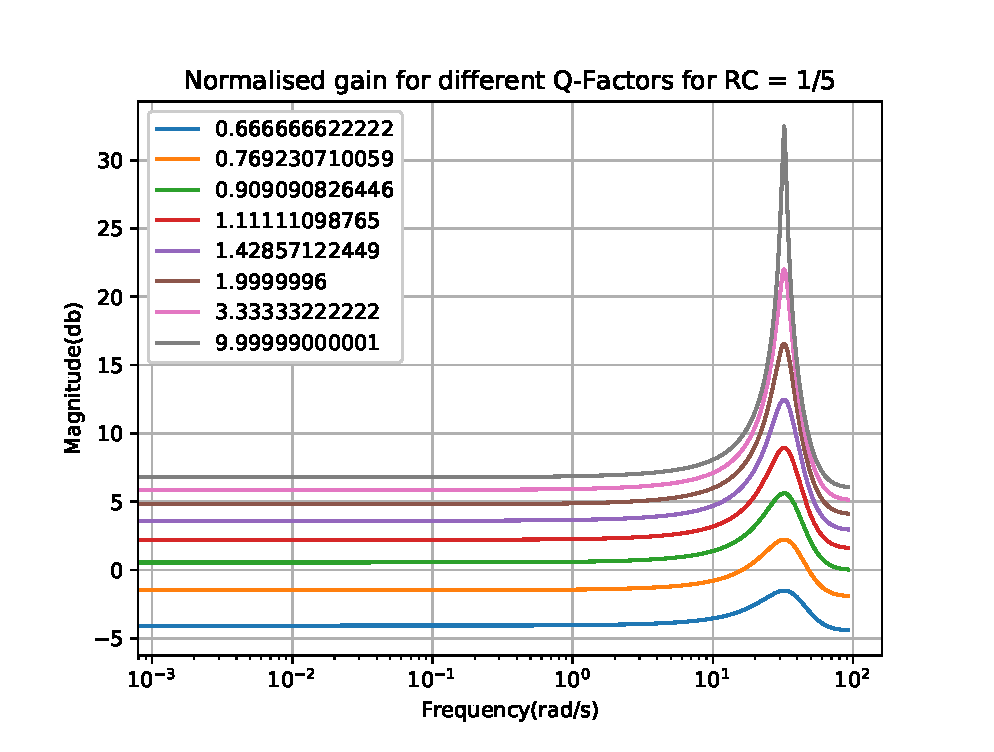
\includegraphics[width=\columnwidth]{./figs/ee18btech11030/ee18btech11030_fc.eps}
\caption{}
\label{fig:ee18btech11030_fig3} 
\end{figure}

The following is code for the plot
\begin{lstlisting}
codes/ee18btech11030/ee18btech11030.py
\end{lstlisting}
From Figure:\ref{fig:ee18btech11030_fig3} ,
\begin{itemize}
\item It is observed that maximally flat response is obtained when Q = 0.71
\item It will be seen that response of the feedback amplifier under consideration shows almost no peaking for Q$\leq$ 0.71 
\end{itemize}
\item Sketch a Pole-Zero Plot to Eq:\ref{eq:ee18btech11030_5} for a varying K

\solution :
\begin{figure}[!ht]
\centering
  \includegraphics[width=\columnwidth]{./figs/ee18btech11030/ee18btech11030_fc1.eps}
\caption{}
\label{fig:ee18btech11030_fig4} 
\end{figure}

The following is code for the  plot
\begin{lstlisting}
codes/ee18btech11030/ee18btech11030_1.py
\end{lstlisting}
From Figure : \ref{fig:ee18btech11030_fig4} 
\begin{itemize}
\item For K = 0,the poles have Q = 0.476 and therefore located on negative real axis. 
\item As K increases poles are brought closer together and eventually coincide at K = 0.1 and Q = 0.5
\item Further increase in K results in poles becoming complex conjugate 
\item Maximally flat response is obtained when Q = 0.707,which results when K = 0.686.In this case poles are at 45\degree .
\item Oscillating response is obtained when poles are completely imaginary when Q = inf which results when K = 2.1 
\end{itemize}

\begin{table}[!ht]
\centering
 
\usetikzlibrary{decorations.markings}
\begin{circuitikz}
\draw (-4,-1) to[amp,t={+K}] (2.5,-1);
\draw (-4,-1) to (-4,2) to (-3,2) ;
\draw (-3,2)  to [capacitor=$C/10$](-3,0.5) to  (-3,0.5) node[ground]{};
\draw (-3,2) to (-2.3,2)to [R=$10R$] (-1.3,2)to (0,2) to [R=$R$] (0,5) node[label={}]{}  to (-4,5) ;
\draw (0,2) to(1,2) to  [capacitor=$C$](1.5,2) to (2.5,2) to (2.5,-1);
\draw (-4,5) to (-4,4.7) to [V=$V_s$] (-4,3.9) to (-4,3.5) node[ground]{} ;
\draw (2.5,-1) to[short, -o] (3,-1) node[label={above:$V_{out}$}]{};
\end{circuitikz}
\caption{}
\label{table:ee18btech11030_table}
\end{table}

\item Building gain K in spice simulation for circuit Fig: \ref{fig:ee18btech11030_fig1}

\solution :

\begin{itemize}
\item For K greater than 1(K = 2.1),the gain block is built using LM741 op-amp.
\begin{figure}[!ht]
	\begin{center}
		\resizebox{\columnwidth/1}{!}{\usetikzlibrary{decorations.markings}
\begin{circuitikz}
\draw (2,2)  node[op amp] (OA) {};
\draw (OA.+) -- (0,1.5) to (0,0) node[label={below:$V_i$}]{};
\draw (OA.-) -- (0,2.5) node[label={}]{} to[R,l_=$R_1$] (-2,2.5) node[ground](GND){};
\draw (OA.out) -- (3,2) node[label={}]{};
\draw (3,2) -- (4.5,2) node[label={above:$V_{o}$}]{};
\draw (3,2) -- (3,4.5) to[R=$R_2$] (0,4.5) -- (0,2.5);
\end{circuitikz}}
	\end{center}
	\caption{LM741 op-amp}
	\label{fig:ee18btech11030_fig5}
\end{figure}
\begin{align}
K = 1 + \frac{R_2}{R_1}
\implies \frac{R_2}{R_1} = 1.1
\end{align}
\item For K less than 1, the gain block is built using voltage divider circuit.
\begin{figure}[!ht]
	\begin{center}
		\resizebox{\columnwidth/1}{!}{\usetikzlibrary{decorations.markings}
\begin{circuitikz}
\ctikzset{tripoles/mos style/arrows}
\draw (1,2) to[short, -o] (0,2) node[label={above:$V_i$}]{};
\draw (1,2) to[R=$R_1$] (2,2) -- (3,2) to[R=$R_2$] (3,0) node[ground](GND){};
\draw (3,2) to[short, -o] (4,2) node[label={above:$V_o$}]{};
\end{circuitikz}}
	\end{center}
	\caption{Voltage Divider}
	\label{fig:ee18btech11030_fig6}
\end{figure}
\begin{align}
K = \frac{R_2}{R_1+R_2}
\end{align}
\end{itemize}

\item Verify the response in time domain using parameters in Table : \ref{table:ee18btech11030_table1} for K = 2.13

\solution :
\begin{figure}[!ht]
\centering
  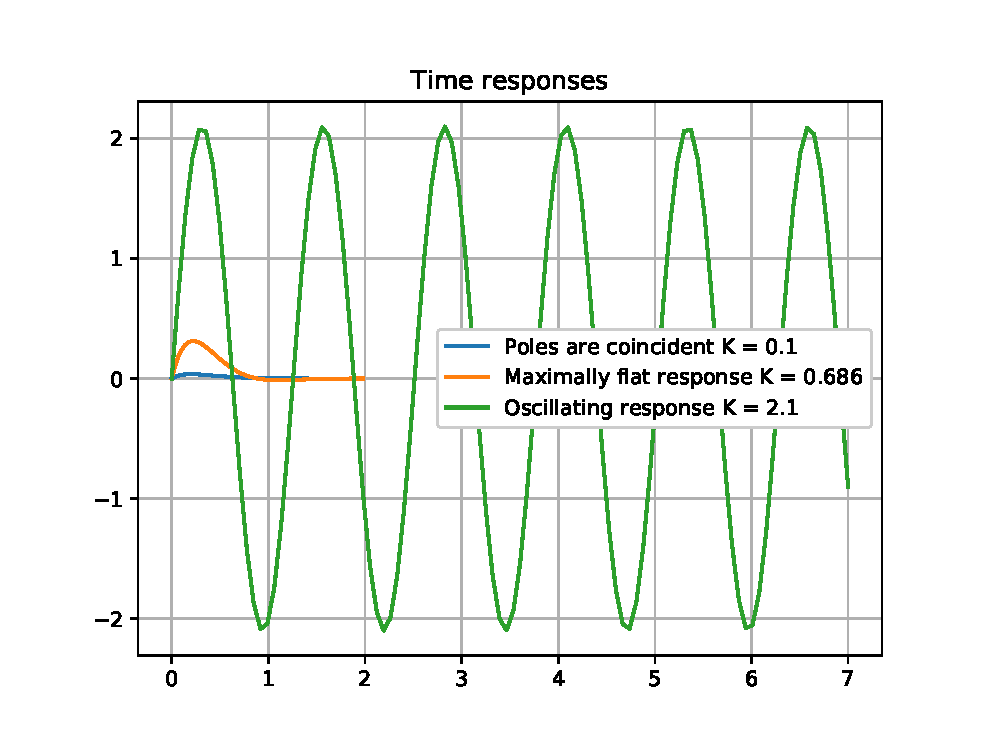
\includegraphics[width=\columnwidth]{./figs/ee18btech11030/ee18btech11030_fc2.eps}
\caption{}
\label{fig:ee18btech11030_fig7} 
\end{figure}

The following is code for the plot
\begin{lstlisting}
codes/ee18btech11030/ee18btech11030_2.py
\end{lstlisting}

\item Choose the appropriate values of R and C to simulate the circuit for K = 2.1

\solution:
\begin{table}[!ht]
\centering
\usetikzlibrary{decorations.markings}
\begin{circuitikz}
\draw (-2,0) to[amp,t={+K}] (3,0);
\draw (3,0) to (3,4) to [capacitor=$C$](1.7,4) to (1,4)  to [R=$R$] (1,2) to (1,2) node[ground]{} ;
\draw (3,4) to [short, -o] (3.5,4) node[label={above:$V_{1}$}]{} ;
\draw [dashed] (2.8,1) to (-1.5,1) to (-1.5,4.5) to (2.8,4.5) to (2.8,1); 
\draw (1,4) to  [R=$10R$] (-1,4) to [capacitor=$C/10$](-1,2) to (-1,2) node[ground]{} ;
\draw (-1,4) to [short, -o] (-2,4) node[label={above:$V_{r}$}]{};
\draw (-2,0) to [short, -o] (-3,0) node[label={above:$V_{t}$}]{} ;
\end{circuitikz}

\caption{}
\label{table:ee18btech11030_table1}
\end{table}
\item Verify the response using the spice model

\solution :

\begin{itemize}
    \item Figure \ref{fig:ee18btech11030_fig8} is the spice simulated output for K = 2.1 using Table \ref{table:ee18btech11030_table1} parameters.
    \item The following is the netlist for simulated circuit.
\begin{lstlisting}
spice/ee18btech11030/ee18btech11030.net
\end{lstlisting}
    \item The following is code for generating output
\begin{lstlisting}
spice/ee18btech11030/ee18btech11030.py
\end{lstlisting}
    
\end{itemize}
\begin{figure}[!ht]
\centering
  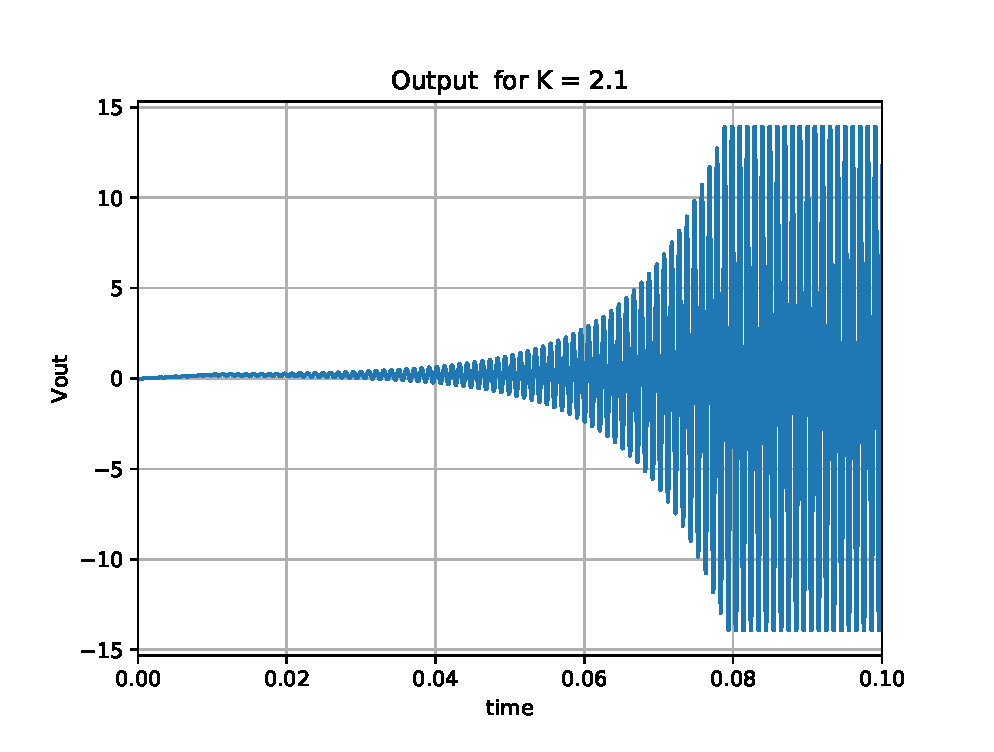
\includegraphics[width=\columnwidth]{./figs/ee18btech11030/ee18btech11030_spice_fc3.eps}
\caption{}
\label{fig:ee18btech11030_fig8} 
\end{figure}

\item Choose the appropriate values of R and C to simulate the circuit for K = 0.1 and K = 0.686

\solution :

\begin{table}[!ht]
\centering
 
\tikzstyle{block} = [draw, fill=white!20, rectangle, 
    minimum height=2em, minimum width=6em]
\tikzstyle{sum} = [draw, fill=white!20, circle, node distance=1cm]
\tikzstyle{input} = [coordinate]
\tikzstyle{output} = [coordinate]
\tikzstyle{pinstyle} = [pin edge={to-,thin,black}]

\begin{tikzpicture}[auto, node distance=3cm,>=latex']
    \node [input, name=input] {};
    \node [sum, right of=input] (sum) {};
    \node [block, right of=sum] (controller) {$G(s) = K$};
    \node [output, right of=controller] (output) {};
    \node [block, below of=controller] (feedback) {$H(s) = \frac{1}{sRC + \frac{1}{sRC} + 2.1}$};

    \draw [->] (sum) -- node {$V_i$} (controller);
    \draw [->] (controller) -- node [name=y] {$V_o$}(output);
    \draw [->] (y) |- (feedback);
    \draw [->] (feedback) -| node[pos=0.99]{$+$}  node [near end] {$V_f$} (sum);
\end{tikzpicture}
\caption{}
\label{table:ee18btech11030_table2}
\end{table}
\item Verify the response using the spice model

\solution 

\begin{figure}[!ht]
\centering
  \includegraphics[width=\columnwidth]{./figs/ee18btech11030/ee18btech11030_spice_fc4.eps}
\caption{}
\label{fig:ee18btech11030_fig9} 
\end{figure}

\begin{itemize}
    \item Figure \ref{fig:ee18btech11030_fig9} is the spice simulated output for K = 0.686 using Table \ref{table:ee18btech11030_table2} parameters.
    \item The following is the netlist for simulated circuit.
\begin{lstlisting}
spice/ee18btech11030/ee18btech11030_1.net
\end{lstlisting}
    \item The following is code for generating output
\begin{lstlisting}
spice/ee18btech11030/ee18btech11030_1.py
\end{lstlisting}
\end{itemize}
\begin{figure}[!ht]
\centering
  \includegraphics[width=\columnwidth]{./figs/ee18btech11030/ee18btech11030_spice_fc5.eps}
\caption{}
\label{fig:ee18btech11030_fig10} 
\end{figure}
\begin{itemize}
    \item Figure \ref{fig:ee18btech11030_fig10} is the spice simulated output for K = 0.1 using Table \ref{table:ee18btech11030_table2} parameters.
    \item The following is the netlist for simulated circuit.
\begin{lstlisting}
spice/ee18btech11030/ee18btech11030_2.net
\end{lstlisting}
    \item The following is code for generating output
\begin{lstlisting}
spice/ee18btech11030/ee18btech11030_2.py
\end{lstlisting}
\end{itemize}
\end{enumerate}
